% !TeX spellcheck = de_DE

\chapter{Methodologies}
\label{chap:k2}

The following sections introduce the principles of 3D lane marking reconstruction method of this work, with the work flow shown in \cref{fig:FlowChart}.

\cref{sec:LineExtraction} describes the applied standard line detection algorithm for labeling the lane markings. To relate the object coordinates of a point with its image coordinates, \cref{sec:Geometry} introduces the imaging properties of aerial images and their mathematical models, including the collinearity equation and lens distortion correction.

\cref{sec:LineFitting} presents the principle of line fitting and further derives the non-linear \gls{ls} model for line equations in two-point form. With the combination of the extended collinearity equation introduced in \cref{sec:Geometry}, \cref{sec:LSadj} elaborates the usage of line fitting for 3D lane marking reconstruction.% The key challenge is to solve the line fitting problem given weakly-textured environments around lane markings and to solve the quasi-infinite line reconstruction problem.

In \cref{sec:LineProjectionOnDSM} the problem of acquiring initial values is described, as initial values of unknown quantities are required in non-linear LS model. Section2.7??? demonstrates how the corresponding measurements in image space are collected given the initial values in object space.

\begin{figure}
  \centering
  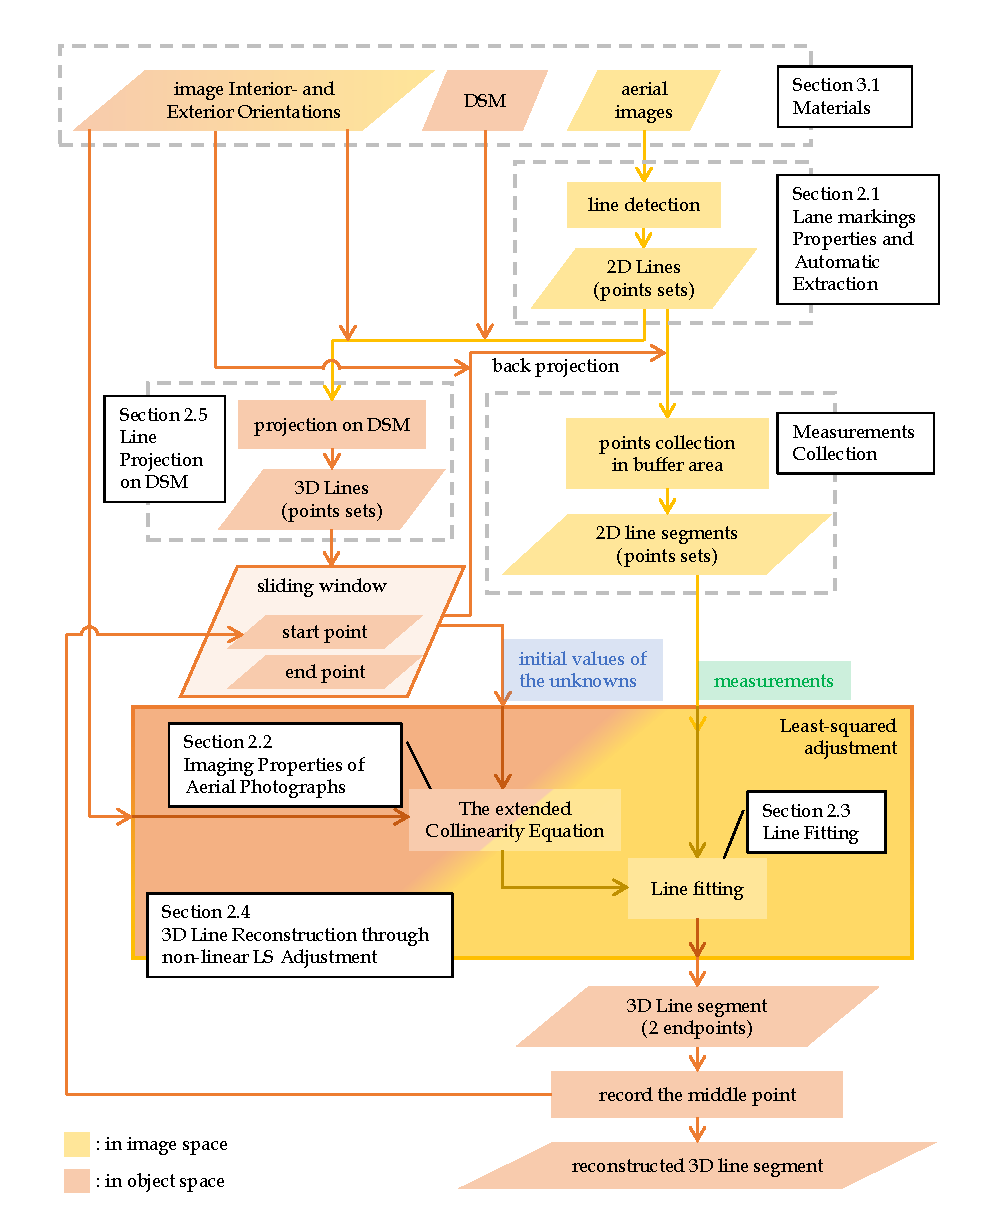
\includegraphics[width=\textwidth]{workflow.pdf}
  \caption{\small The work flow}
  \label{fig:FlowChart}
\end{figure}

\clearpage


%%%%%%%%%%%%%%%%%%%%%%%%%%%%%%%%%%%%%%%%%%%%%%%%%%%%%%%%
\section{Lane markings Properties and Automatic Extraction}
\label{sec:LineExtraction}
% Missing some small review about alternative methods?
% This chapter should be much more detailled.
The appearance of lane markings on German roads including line type, color and width is specified depending on the road type. Different line types of lane markings are shown in \cref{fig:LaneMarkingTypes} and their line widths are defined in \cref{tab:LaneMarkingWidths}.
% https://de.wikipedia.org/wiki/Fahrbahnmarkierung#Eigenschaften
% Richtlinien für die Markierung von Straßen (RMS) Teil 1

Because of the appearance, the problem of lane marking detection can be treated as a line detection problem. We restrict the proposed framework to lane markings with single white lines (dashed or continuous) of 0.3 meter width. Other types like in restricted zone, double lines, parking areas, temporal yellow lines in construction sites etc, are excluded. % https://www.transchool.lee.army.mil/adso/documents/zeichen.pdf

The principle to extract line features is to firstly derive the line direction for each pixel by using partial derivatives of a Gaussian smoothing kernel. Pixels that have a local maximum in the second directional derivative perpendicular to the line direction are marked as line points. By thresholding their second directional derivative values, the accepted line points are then linked and connected.
% C. Steger: “Extracting Curvilinear Structures: A Differential Geometric Approach”. In B. Buxton, R. Cipolla, eds., “Fourth European Conference on Computer Vision”, Lecture Notes in Computer Science, Volume 1064, Springer Verlag, pp. 630-641, 1996. 
% C. Steger: “Extraction of Curved Lines from Images”. In “13th International Conference on Pattern Recognition”, Volume II, pp. 251-255, 1996. 
% C. Steger: “An Unbiased Detector of Curvilinear Structures”. IEEE Transactions on Pattern Analysis and Machine Intelligence, vol. 20, no. 2, pp. 113-125, 1998
The resultant connected points which compose a line are of sub-pixel precision. \cref{fig:LineExtraction} shows the extracted lines on the original image.
% http://www.mvtec.com/doc/halcon/11/en/lines_gauss.html

\begin{figure}
\centering
\subfloat[\small Continuous line]{\fbox{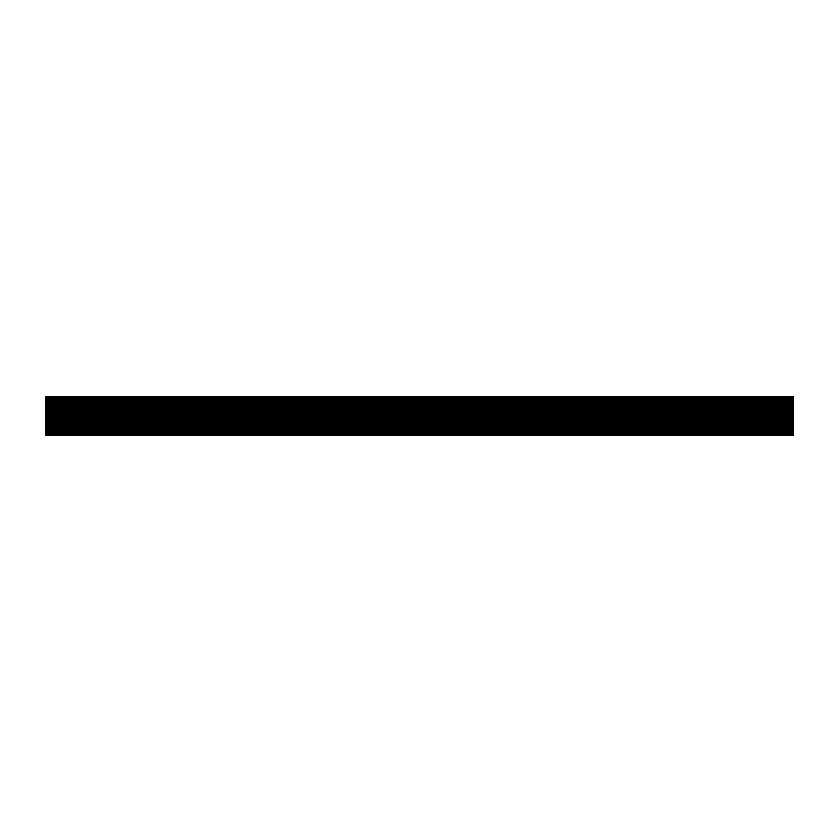
\includegraphics[width=0.3\textwidth, trim={0 150 0 150},clip=true]{Laengsmarkierung_durchgehend.pdf}}}
\quad
\subfloat[\small Dashed line]{\fbox{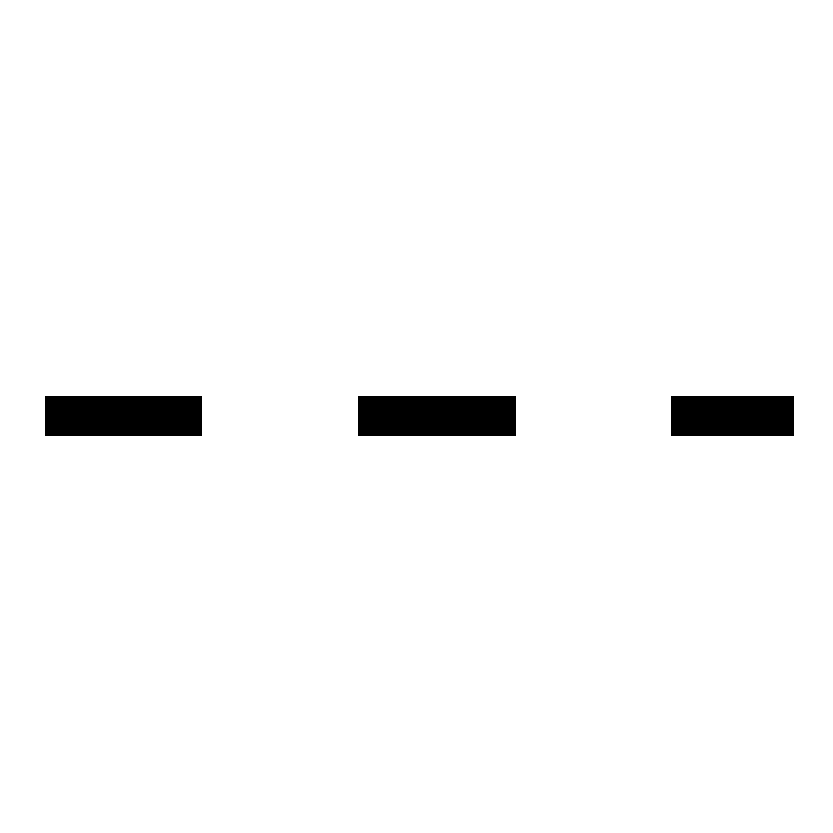
\includegraphics[width=0.3\textwidth, trim={0 150 0 150},clip=true]{Laengsmarkierung_unterbrochen.pdf}}}
\newline
\subfloat[\small Continuous and dashed double lines]{\fbox{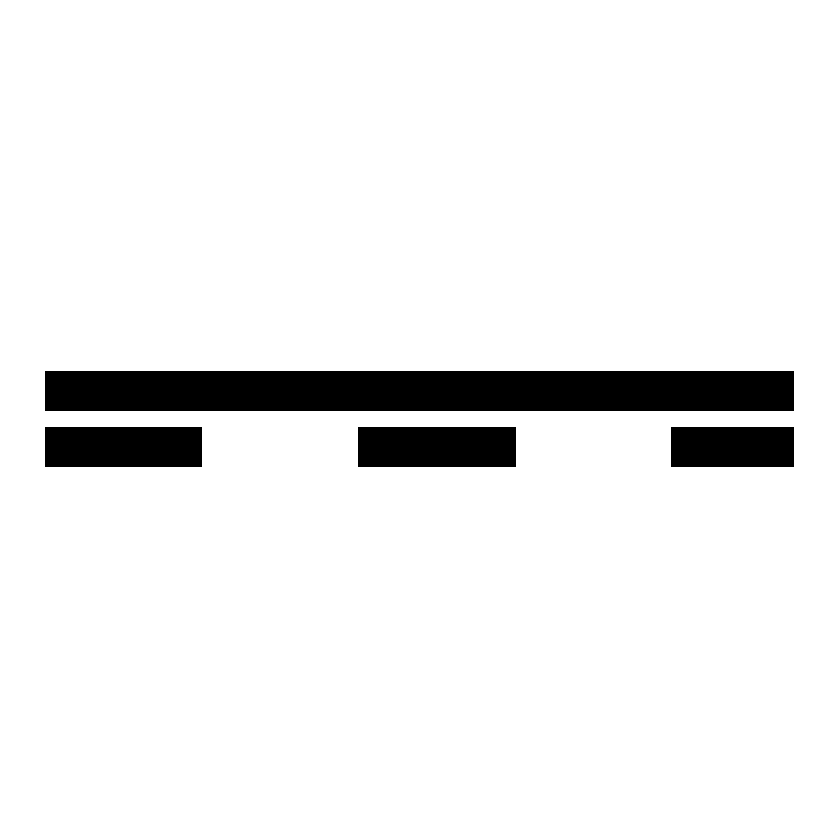
\includegraphics[width=0.3\textwidth, trim={0 150 0 150},clip=true]{Laengsmarkierung_unterbrochen_durchgehend.pdf}}}
\quad
\subfloat[\small Continuous double lines]{\fbox{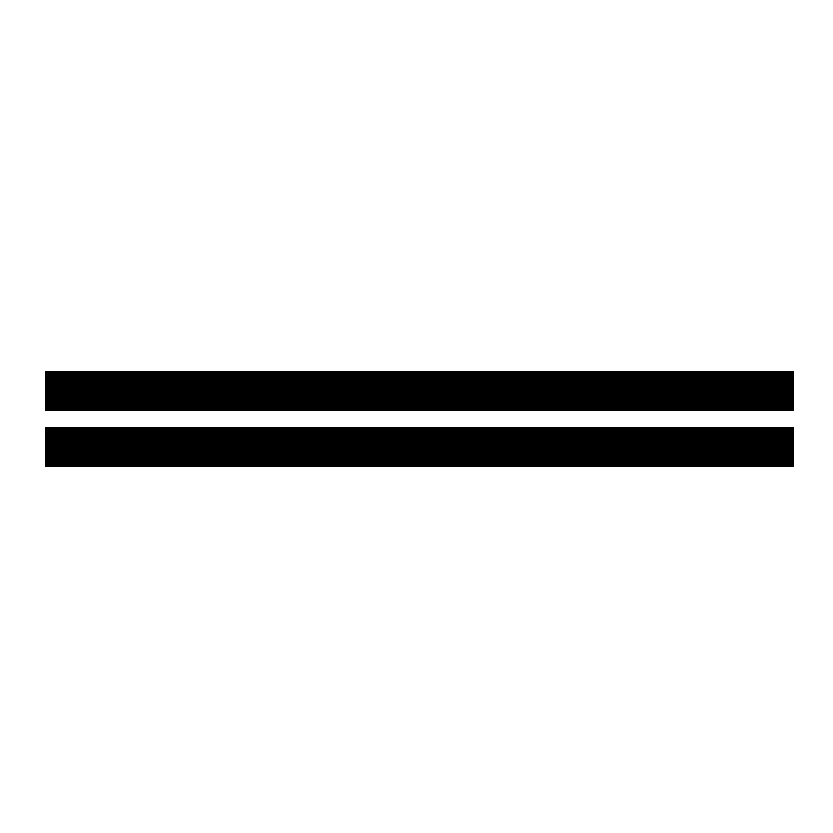
\includegraphics[width=0.3\textwidth, trim={0 150 0 150},clip=true]{Laengsmarkierung_durchgehend_doppelt.pdf}}}
\quad
\subfloat[\small Dashed double lines]{\fbox{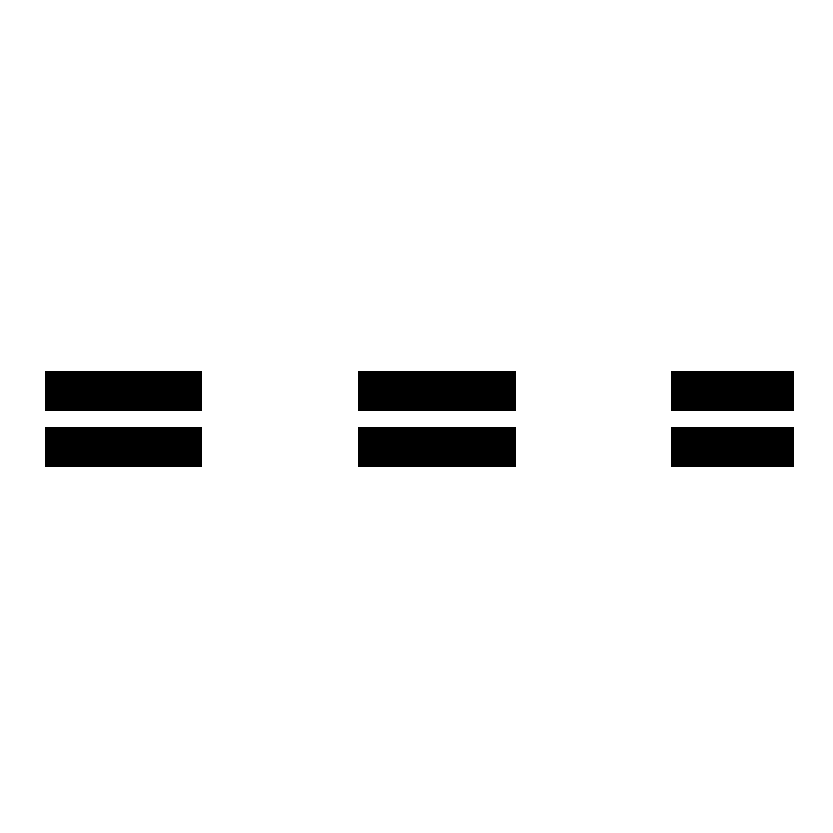
\includegraphics[width=0.3\textwidth, trim={0 150 0 150},clip=true]{Laengsmarkierung_unterbrochen_doppelt.pdf}}}
\caption{\small Line types of lane markings [source RMS Teil 1]}
% https://de.wikipedia.org/wiki/Fahrbahnmarkierung
% Richtlinien für die Markierung von Straßen (RMS) Teil 1

\label{fig:LaneMarkingTypes}
\end{figure}
\setlength{\floatsep}{20pt plus 1.0pt minus 2.0pt}
\begin{table}
    \centering
    \begin{tabular}{l|cc}
    \toprule
           & motorways\footnote{and corresponding roads in the sense of the VwV-StVO to § 42 to mark 330 (motorway) II}  & other roads\\
    \midrule
    narrow lines & $0.15$ [m] & $0.12$ [m] \\
    wide lines   & $0.30$ [m] & $0.25$ [m] \\
    \bottomrule
    \end{tabular}
    \caption{\small Line widths of lane markings [source RMS Teil 1]}
    \label{tab:LaneMarkingWidths}
% Der Deutsche Verkehrssicherheitsrat
% https://www.dvr.de/download/publikationen-schriftenreihe-17.pdf
% Richtlinien für die Markierung von Straßen (RMS) Teil 1
\end{table}


\begin{figure}
  \centering
  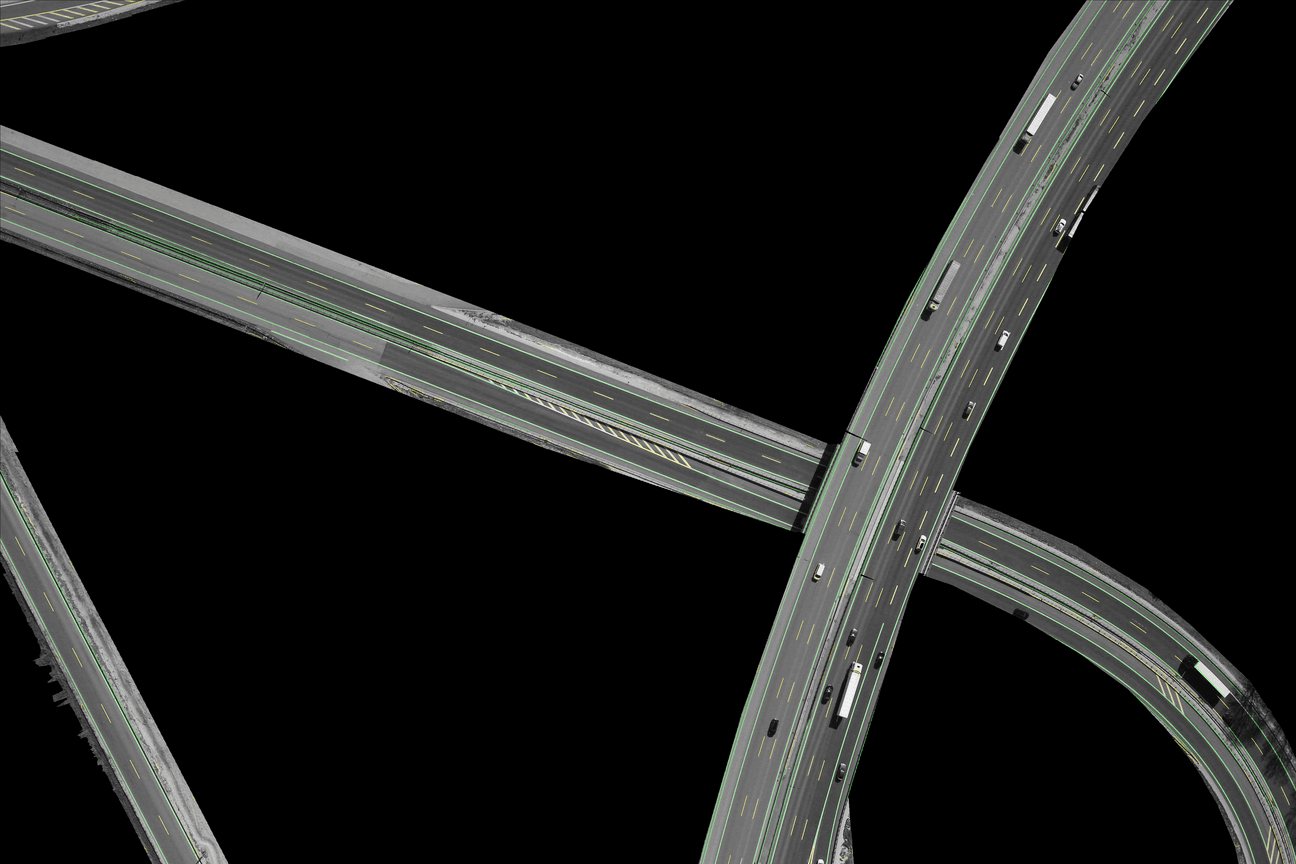
\includegraphics[width=0.7\textwidth, trim=750 250 200 320,clip]{ML1234_extlines_rsz.png}
  \caption{\small Lane markings Extraction. The extracted long lane-lines are marked in green and the dashed ones are in yellow.  Note that both cases are reconstructed into 3D with the same framework; different colors here are only for illustration.}
  \label{fig:LineExtraction}
\end{figure}



%%%%%%%%%%%%%%%%%%%%%%%%%%%%%%%%%%%%%%%%%%%%%%%%%%%%%%%%
\section{Imaging Properties of Aerial Photographs}
\label{sec:Geometry}

This section describes the geometric model of the projection of 3D points into the image generated by a real camera. We first restrict the discussion in \cref{subsec:Collinearity} to central perspective projection where the collinearity equation originate from. We then model deviations from this model, addressing real cameras with imperfect lenses, in \cref{subsec:LensDistortion}.

\subsection{Collinearity Equations}
\label{subsec:Collinearity}
We assume frame photography, i.e. photographs exposed on a frame chip in one instant, and assume central projection model with cameras that have a single viewpoint and a planar sensor and being straight line-preserving. Collinearity indicates the condition that the image point (on the sensor plate of the camera), the observed point (in object space) and the projection center of the camera were aligned at the moment the picture was taken. Every measured point leads to two collinearity equations, describing transformations from object space to image coordinates:
\begin{equation} \label{eq:collinearity}
\begin{split}
x = x_0 -c \dfrac {R_{11}(X-X_0) + R_{21}(Y-Y_0) + R_{31}(Z-Z_0)} {R_{13}(X-X_0) + R_{23}(Y-Y_0) + R_{33}(Z-Z_0)} \\
y = y_0 -c \dfrac {R_{12}(X-X_0) + R_{22}(Y-Y_0) + R_{32}(Z-Z_0)} {R_{13}(X-X_0) + R_{23}(Y-Y_0) + R_{33}(Z-Z_0)}
\end{split}
\end{equation}
where\newline
$(x, y)$: image coordinates of the point \newline
$(x_0, y_0)$: image coordinates of principal point \newline
$c$: principal distance; focal length \newline
$(X, Y, Z)$: object coordinates of the point \newline
$(X_0, Y_0, Z_0)$: object coordinates of projection center \newline
$R_{11},...,R_{33}$: elements of the rotation matrix R (orthogonal 3$\times$3-matrix from object space to image space, with 3 independent angles $\omega$, $\phi$ and $\kappa$)

\subsection{Lens Distortion Correction}
\label{subsec:LensDistortion}

An original image appears to have some degree of deviations from perspective mapping due to lens distortion, lens refraction or non-planarity of the sensor surface. There are several models to describe these perturbing effects and can be used to undistort the images, resulting in rectified images which are now straight line-preserving.
 
A 6-parameter lens distortion model is chosen, with two radial symmetric distortion parameters $A_1$ and $A_2$, two asymmetric parameters $B_1$ and $B_2$, and a scaling $C1$ and an affine shearing parameter $C_2$. Assuming $x$ and $y$ to be the distorted image coordinates, the corrections $\Delta x$ and $\Delta y$ are then calculated by the following equations:
\begin{equation} \label{eq:LensDistortion}
\begin{split}
\Delta x &= x_p + A_1x_*(r^2-R_0^2) + A_2x_*(r^4-R_0^4) + B_1(r^2+2x_*^2) + B_22x_*y+C_2y \\
\Delta y &= y_p + A_1y  (r^2-R_0^2) + A_2y  (r^4-R_0^4) + B_1(r^2+2y^2)   + B_22x_*y
\end{split}
\end{equation}
with $r=\sqrt{x_*^2+y^2}$ and $x_*=\dfrac{x}{C_1}$.

The undistorted image coordinates $x\prime$ and $y\prime$ are then calculated by
\begin{equation} \label{eq:undistortedimgcoord}
\begin{split}
x\prime=x+\Delta x \\
y\prime=y+\Delta y
\end{split}
\end{equation}
 [F. Kurz et al. 2012] 
% The reference is not the original one

\subsection{Extended Collinearity Equation}
\label{subsec:ExtendedCollinearity}
As real cameras generally only approximate the perspective camera model, lens distortion correction can be additionally included in the collinearity model, attempting to correct the pixel position so that they obey the perspective model with sufficient accuracy.[W. Förstner et al. 2016] 
% The reference is not the original one

By inserting \cref{eq:collinearity} and \cref{eq:LensDistortion} into \cref{eq:undistortedimgcoord} , the relationship between a 3D point $\mathbf{P}(X, Y, Z)$ and its corresponding distorted image coordinates $\mathbf{p}(x\prime,y\prime)$ can be described as
\begin{equation} \label{eq:expandedcollinearity}
\begin{split}
x =& x_0-c\dfrac{R_{11}(X-X_0)+R_{21}(Y-Y_0)+R_{31}(Z-Z_0)}{R_{13}(X-X_0)+R_{23}(Y-Y_0)+R_{33}(Z-Z_0)} \\
&-(x_p + A_1x_*(r^2-R_0^2) + A_2x_*(r^4-R_0^4) + B_1(r^2+2x_*^2) + B_22x_*y+C_2y)\\
y =& y_0-c\dfrac{R_{12}(X-X_0)+R_{22}(Y-Y_0)+R_{32}(Z-Z_0)}{R_{13}(X-X_0)+R_{23}(Y-Y_0)+R_{33}(Z-Z_0)} \\
&-(y_p + A_1y  (r^2-R_0^2) + A_2y  (r^4-R_0^4) + B_1(r^2+2y^2)   + B_22x_*y)
\end{split}
\end{equation}

To simplify the representation: a function $\mathcal{G}$ which takes the interior and exterior orientations as well as the lens distortion parameters of a camera $\mathbf{q}(x_0,y_0,c,X_0,Y_0,Z_0,R_{11},...,R_{33},A_1,A_2,B_1,B_2,C_1,C_2)$ and takes the position of a 3D point $\mathbf{P}(X, Y, Z)$, and returns the corresponding distorted image coordinates $\mathbf{p}(x,y)$, can be shortly expressed by
\begin{equation} \label{eq:Gfunction}
\mathbf{p} = \mathcal{G}(\mathbf{q},\mathbf{P}) 
\end{equation}

%%%%%%%%%%%%%%%%%%%%%%%%%%%%%%%%%%%%%%%%%%%%%%%%%%%%%%%%
\section{Line Fitting}
\label{sec:LineFitting}

Line fitting is the process of constructing a infinite straight line that has the best fit to a 2D dataset. One of the approaches is linear regression which attempts to model the relationship between two variables by fitting a linear equation to observed data. % [www.stat.yale.edu/Courses/1997-98/101/linreg.htmf]
Additional least-squares (LS) models are commonly used for regression by means of minimization of sum of squared residuals.

In the case of simple linear regression as presented in \cref{subsec:LinearRegression}, the independent variable $x$ is error free, inconsistencies are only for the dependent variable $y$. Geometrically it means that the vertical distances from observed data to the fitted line is minimized. To minimize the sum of squared perpendicular distances from the data points to the regression line, a LS mixed model is derived in \cref{subsec:MixedModel} to perform orthogonal regression.

For a later combination with point-wise extended collinearity equation \eqref{eq:Gfunction} in next section, we aim to fit the line equation in two-point form to the extracted lines produced in \cref{sec:LineExtraction} (in forms of sets of points in image coordinates). For such non-linear least squares fitting purpose, a non-linear mixed model is derived in \cref{subsec:NonLinear}. 


\subsection{Linear Regression}
\label{subsec:LinearRegression}

Given a data set $\{x_i,y_i\}^n_{i=1}$ of $n$ points on a 2D plane, a linear regression model assumes that the relationship between the dependent variable $y_i$ and the regressors $x_i$ is linear. This relationship is modeled through a error variable $e_{y_i}$--- an unobserved random variable that adds noise to the linear relationship between the dependent variable and regressors.
Thus the model takes the form:
\begin{equation} \label{eq:SimpleLinearRegression}
y_i - e_{y_i} = a_0 + a_1x_i
\end{equation}
where $a_0$ and $a_1$ are the regression coefficients.
%https://en.wikipedia.org/wiki/Linear_regression#Assumptions


\subsection{Orthogonal Regression ---Mixed Model}
\label{subsec:MixedModel}

In the case with inconsistencies $e_{x_i}$ and $e_{y_i}$ in both observations $x_i$ and $y_i$, A-model with pseudo observation equations can be adopted and the observation equations are formulated:
\begin{equation} \label{eq:MixModel1-1}
y_i - e_{y_i} = a_0 + a_1(x_i-e_{x_i}) = a_0 + a_1\bar{x_i}
\end{equation}
\begin{equation} \label{eq:MixModel1-2}
x_i-e_{x_i} = \bar{x_i}
\end{equation}

In the A-model, every observation is either a linear or a non-linear function of all unknown quantities. In contrast, in the B-model no unknown parameter exist and there are linear or non-linear relationships between the observations [F. Krumm]. As \eqref{eq:MixModel1-1} describes the relationship between observations and unknowns and \eqref{eq:MixModel1-2} describes the relationship between observations, this model is known as the mixed model or Gauss-Helmert model.


\subsection{Non-linear Mixed Model}
\label{subsec:NonLinear}

Line Equation in two-point form:
\begin{equation} \label{eq:LineInTwoPointForm}
y-y_1 = \dfrac{(y_2-y_1)}{(x_2-x_1)}\times(x-x_1)
\end{equation}
where two points $(x_1,y_1)$ and $(x_2,y_2)$ define the infinite line with $x_2\neq x_1$, and $(x,y)$ is any point on the line.

Let the unknown image coordinates of the endpoints of a line be $(x_1,y_1)$ and $(x_2,y_2)$, and the inconsistent observations $\{x_i,y_i\}^n_{i=1}$. The model of observation equations \eqref{eq:MixModel1-1} and \eqref{eq:MixModel1-2} now takes the form: 
\begin{equation} \label{eq:MixModel2-1}
y_i - e_{y_i}= (y_1-\dfrac{(y_2-y_1)}{(x_2-x_1)}\times x_1) + \dfrac{(y_2-y_1)}{(x_2-x_1)}\times \bar{x_i}
\end{equation}
\begin{equation} \tag{\ref{eq:MixModel1-2} revisited}
x_i-e_{x_i} = \bar{x_i}
\end{equation}
Each observation $y_i$ in \eqref{eq:MixModel2-1} is a non-linear function of all unknown quantities.

A functions $\mathcal{F}$ which takes two image points $\mathbf{u}$ and $\mathbf{v}$ that define an infinite line, and takes the measured x coordinate $\mathbf{p_x}$ of an image point $\mathbf{p}$, and returns the estimated image coordinates $\mathbf{\hat{p}}$ which lies on the infinite line $\overline{\mathbf{u}\mathbf{v}}$, can be shortly expressed by
\begin{equation} \label{eq:Ffunction}
\mathbf{\hat{p}} = \mathcal{F}(\mathbf{u},\mathbf{v},\mathbf{p_x})
\end{equation}
Note that as a combination of \eqref{eq:MixModel2-1} and \eqref{eq:MixModel1-2}, function $\mathcal{F}$ is actually composed of
\begin{equation} \label{eq:Ffunction_xy}
\begin{split}
\mathbf{\hat{p}_x} = \mathcal{F}^x(\mathbf{u},\mathbf{v},\mathbf{p_x})\\
\mathbf{\hat{p}_y} = \mathcal{F}^y(\mathbf{u},\mathbf{v},\mathbf{p_x})
\end{split}
\end{equation}

% % %
% which can be further rewritten:
%forms the observation equation
%Taylor expansion...(local linear approximation)
%the linear equation can also be expanded

\clearpage
%%%%%%%%%%%%%%%%%%%%%%%%%%%%%%%%%%%%%%%%%%%%%%%%%%%%%%%%
\section{3D line reconstruction through non-linear LS Adjustment}
\label{sec:LSadj}

In this section, we aim to refine the position of a 3D line segment so that its back-projection in each covering image has a best-fit to the extracted line. To simplify the problem, a long curved lane-line is partially reconstructed through a sliding window. It is approximated by a straight line of 9 meters in length, taking into account the maximum curvature of the highway.

In a sliding window of 9 meters length, a line segment is reconstructed with the measurements collected in the corresponding regions (with buffer width 5 pixels) on all covering images. Only the middle point of this reconstructed 3D line is recorded. The sliding window then moves 4.5 meters forward, started from the recorded middle point of the previous line segment. Another line segment is then reconstructed, with its middle point being recorded... and so on. These recorded middle points are in the end the nodes of the reconstructed line. The reconsideration in overlapping region makes the reconstruction more robust.

In \cref{subsec:ObsEqua} we firstly set-up a model of observation equations. It describes the fitting of a straight line to the measurements on each covering images, where the fitting lines on different images are transformed from a single 3D straight line segment through extended collinearity equation.

Regarding the fact that the collinearity is a point-wise condition, a line segment is represented by its two endpoints whose object coordinates are the six unknown parameters in our LS model. Correspondingly, the observation equations are line equations in two-point form. A Line equation has however a mathematical meaning of infinite length. Therefore, some constraints on unknowns are necessary to avoid arbitrary locations of the two points on the infinite reconstructed 3D line. The constraint equations are modeled in \cref{subsec:ConEqua}.




%Additionally, the measurements are collected accordingly.

%infinitely many solutions.

\subsection{Model of Observation Equations}
\label{subsec:ObsEqua}

Given the start-point $P_s(X_s,Y_s,Z_s)$ and the end-point $P_e(X_e,Y_e,Z_e)$ of a line segment in object space. Consider the case where there are $J$ images covering this line segment. With \cref{eq:Gfunction}, the start- and end-points of this line segment's back-projection in image $j$ have the image coordinates $p^j_s(x^j_s,y^j_s)$ and $p^j_e(x^j_e,y^j_e)$:
\begin{equation} \label{eq:obsmodel-collinearity}
\begin{split}
p^j_s = \mathcal{G}(q^j,P_s)\\
p^j_e = \mathcal{G}(q^j,P_e)
\end{split}
\qquad
\begin{split}
\forall j=1,2,...J
\end{split}
\end{equation}

Let $l^j$ be an extracted line on image $j$ where there are $L^j$ extracted lines in this image, and $n^j_{l,i}$ be a point in line $l^j$ where this line consists of $N^j_l$ points. Given a measured x coordinate $n^j_{l,i,x}$ of a point $n^j_{l,i}$, the estimated image coordinates $\hat{n}^j_{l,i}(\hat{x}^j_{l,i},\hat{y}^j_{l,i})$ on the infinite line $\overline{p^j_s,p^j_e}$ computed from \cref{eq:Ffunction} is:
\begin{equation} \label{eq:obsmodel-linefitting}
\hat{n}^j_{l,i} = \mathcal{F}(p^j_s,p^j_e,n^j_{l,i,x})
\qquad
\forall i=1,2,...N^j_l
\end{equation}

Writing \eqref{eq:obsmodel-collinearity} into \eqref{eq:obsmodel-linefitting} gives a function $\mathcal{H}$:
\begin{equation} \label{eq:obsmodel}
\begin{split}
\hat{n}^j_{l,i} &= \mathcal{F}(\mathcal{G}(q^j,P_s),\mathcal{G}(q^j,P_e),n^j_{l,i,x})\\
&=\mathcal{H}(q^j,P_s,P_e,n^j_{l,i,x})
\qquad
\forall i=1,2,...N^j_l,\quad\forall l=1,2,...L^j,\quad\forall j=1,2,...J
\end{split}
\end{equation}
where $n^j_{l,i,x}\quad\forall i=1,2,...N^j_l$ are the measurements, $P_s$ and $P_e$ are the unknowns, $q^j\quad\forall j=1,2,...J$ includes the known interior and exterior orientations of camera $j$.\newline

Correspond to \cref{eq:Ffunction_xy}, function $\mathcal{H}$ is composed of
\begin{equation}
\begin{split}
\hat{n}^j_{l,i,x} = \mathcal{H}^x(q^j,P_s,P_e,n^j_{l,i,x})\\
\hat{n}^j_{l,i,y} = \mathcal{H}^y(q^j,P_s,P_e,n^j_{l,i,x})
\end{split}
\end{equation}

Since the adjustment is done "line-wise"--- for a pair of $P_s$ and $P_e$, the measurements are collected correspondingly. Thus the subscription $l$ representing specific line segment will be left out in the followings.

For an image $j=1$ there are $2\times N^j$ observation equations:

\begin{equation} \label{eq:obs-camera1}
\begin{bmatrix}
n^1_{1,y}\\[0.3em]
n^1_{2,y}\\[0.3em]
...\\[0.3em]
n^1_{N^1,y}\\[0.5em]
n^1_{1,x}\\[0.3em]
n^1_{2,x}\\[0.3em]
...\\[0.3em]
n^1_{N^1,x}
\end{bmatrix}
\doteq % dot equal indicates inconsistency
\begin{bmatrix}
\mathcal{H}^y(q^1,P_s,P_e,n^1_{1,x})\\[0.3em]
\mathcal{H}^y(q^1,P_s,P_e,n^1_{2,x})\\[0.3em]
...\\[0.3em]
\mathcal{H}^y(q^1,P_s,P_e,n^1_{N^1,x})\\[0.5em]
\mathcal{H}^x(q^1,P_s,P_e,n^1_{1,x})\\[0.3em]
\mathcal{H}^x(q^1,P_s,P_e,n^1_{2,x})\\[0.3em]
...\\[0.3em]
\mathcal{H}^x(q^1,P_s,P_e,n^1_{N^1,x})
\end{bmatrix}
\end{equation}

Note that dot equal indicates inconsistency between the measured value, $n^j_i$, and the computed value, $\mathcal{H}^y(q^j,P_s,P_e,n^j_i)$.

For all covering image $j=1,2,...J$ there are $2\times\displaystyle\sum_{j=1}^{J}N^j$ observation equations.

%\begin{equation} \label{eq:obs-cameraJ}
%\begin{bmatrix}
%n^1_{l,i,y}\\[0.3em]
%n^1_{l,i,x}\\[0.3em]
%n^2_{l,i,y}\\[0.3em]
%n^2_{l,i,x}\\[0.3em]
%...\\[0.3em]
%n^J_{l,N^1,y}\\[0.3em]
%n^J_{l,N^1,x}
%\end{bmatrix}
%\doteq % dot equal indicates inconsistency
%\begin{bmatrix}
%\mathcal{H}(q^1,P_s,P_e,n^1_{l,i,y})\\[0.3em]
%\mathcal{H}(q^1,P_s,P_e,n^1_{l,i,x})\\[0.3em]
%\mathcal{H}(q^2,P_s,P_e,n^2_{l,i,y})\\[0.3em]
%\mathcal{H}(q^2,P_s,P_e,n^2_{l,i,x})\\[0.3em]
%...\\[0.3em]
%\mathcal{H}(q^J,P_s,P_e,n^J_{l,i,y})\\[0.3em]
%\mathcal{H}(q^J,P_s,P_e,n^J_{l,i,x})
%\end{bmatrix}
%\end{equation}


\subsection{Model of Constraint Equations}
\label{subsec:ConEqua}
%At least two constraints are needed to fix rank deficiency???. 
There are three constraints used in this work:
\begin{itemize}
\item Fixing the X, Y coordinates of the start-point:
\item [] \begin{equation} \label{eq:constraint1}
\hat{X}^s=X^s_0
\end{equation}
\begin{equation} \label{eq:constraint2}
\hat{Y}^s=Y^s_0
\end{equation}
\item Fixing the length of the line segment (i.e. constraining the relative location of the end-point):
\begin{equation} \label{eq:constraint3}
\sqrt{(\hat{X}^s-\hat{X}^e)^2+(\hat{Y}^s-\hat{Y}^e)^2+(\hat{Z}^s-\hat{Z}^e)^2}=S
\end{equation}
\end{itemize}

Note that only in the first line segment reconstruction of a long lane marking, the fixed $X_s$ and $Y_s$ values are from the approximated initial value derived from \cref{sec:LineProjectionOnDSM}. From the second line segment on, the fixed values $X_s$ and $Y_s$ are from the previously determined values.


\subsection{Non-linear LS Adjustment with Constraints}
\label{subsec:LSadj}

A non-linear equation system is approximated to be locally linear with small step size of the unknown quantities. Through a linearized form of the equation system, for example Taylor's polynomial expansion, it turns to solve for the increments of unknowns instead of the unknowns themselves, where linear LS adjustment is applied iteratively until convergence is achieved. Depending on the configuration and initial parameters chosen, the nonlinear fit may have good or poor convergence properties.



% In this work, both the observation equations and constraint equations are linearized, i.e. all equations are expanded to Taylor's polynomials.



% 2.5.3 non-linear mixed model with constraints...
% 2.5.3.1 The Model and Its Linearization
% local linear
% combine the obs & con model, linearization
% 2.5.3.2 The Solution of the linearized problem

% system solvable when J>1 and well distributed, 





% % %
% derive matrices
% extended normal equation matrix N*


%%%%%%%%%%%%%%%%%%%%%%%%%%%%%%%%%%%%%%%%%%%%%%%%%%%%%%%%
\section{Line Projection on DSM}
\label{sec:LineProjectionOnDSM}

As the equation system in \cref{sec:LSadj} may exhibit multiple local minimum, a "correct" initial approximation of the unknowns is required for convergence to the correct solution. To provide such initial 3D line segment, the extracted line features derived in \cref{sec:LineExtraction} can be projected onto DSM with the bundle adjusted camera orientations.

Given image coordinates $\mathbf{p}(x,y)$ of a point and (bundle-adjusted) image orientations $\mathbf{q}$, there is still one degree of freedom in extended collinearity equation \eqref{eq:Gfunction} on solving object coordinates $\mathbf{P}(X,Y,Z)$. Combined with the usage of DSM, which provides the height information $Z$ given a position $(X,Y)$, the corresponding object coordinates can be solved iteratively until the increment $\Delta Z$ small enough, i.e. convergence achieved.

Considering that the DSM is raster (discrete) whereas $X$ and $Y$ have continuous numerical values, DSM height is bilinear interpolated.

%Given image coordinates of an image point and an initial Z-value $Z_{initial}$, the 
%With the following work flow:

%pseudo code:

%x,y = a set of points (detected line);		// unit: [pixel], in image coordinates
%Z_ini = 500;						// unit: [meter], in world coordinates
%while( ( Z_new – Z_ini ) < convergentthreshold )
%	(X,Y) = camera.img2geo(x,y,Z_ini);	// X,Y in world coordinates
%	Z_new = DSM.Get_height(X,Y);		// Z_new in world coordinates
%end
%return (X,Y,Z_new);

%\begin{Algorithmus} 
%\caption{Line Projection on DSM}
%\label{alg:LineProjectionOnDSM}
%\begin{algorithmic}
%\Procedure{Sample}{$a$,$v_e$}
%  \State $\mathsf{parentHandled} \gets (a = \mathsf{process}) \lor \mathsf{visited}(a'), (a',c,a) \in \mathsf{HR}$
%  \State \Comment $(a',c'a) \in \mathsf{HR}$ denotes that $a'$ is the parent of $a$
%  \If{$\mathsf{parentHandled}\,\land(\mathcal{L}_\mathit{in}(a)=\emptyset\,\lor\,\forall l \in %\mathcal{L}_\mathit{in}(a): \mathsf{visited}(l))$}
%    \State $\mathsf{visited}(a) \gets \text{true}$
%    \State $\mathsf{writes}_\circ(a,v_e) \gets
%    \begin{cases}
%      \mathsf{joinLinks}(a,v_e)                & \abs{\mathcal{L}_\mathit{in}(a)} > 0\\
%      \mathsf{writes}_\circ(p,v_e)             & \exists p: (p,c,a) \in \mathsf{HR}\\
%      (\emptyset, \emptyset, \emptyset, false) & \text{otherwise}
%    \end{cases}
%  \EndIf
%\EndProcedure
%\end{algorithmic}
%\end{Algorithmus}




% % %





%%%%%%%%%%%%%%%%%%%%%%%%%%%%%%%%%%%%%%%%%%%%%%%%%%%%%%%%
%\section{Line Grouping}
%\label{sec:}





%\begin{equation}\label{eq:test}
%a = b + c.
%\end{equation}

%\begin{equation}
%a = b + c. \tag{\ref{eq:test} revisited}
%\end{equation}



